\section{Implementation}

\subsection{User interface}

\subsubsection{New project page}
Form interface allowing users to create a new LaTeX project, with options to set project name, template selection, and initial configuration, as seen in Figure \ref{fig:ui-newproject}.

\begin{figure}[htb]
    \centering
    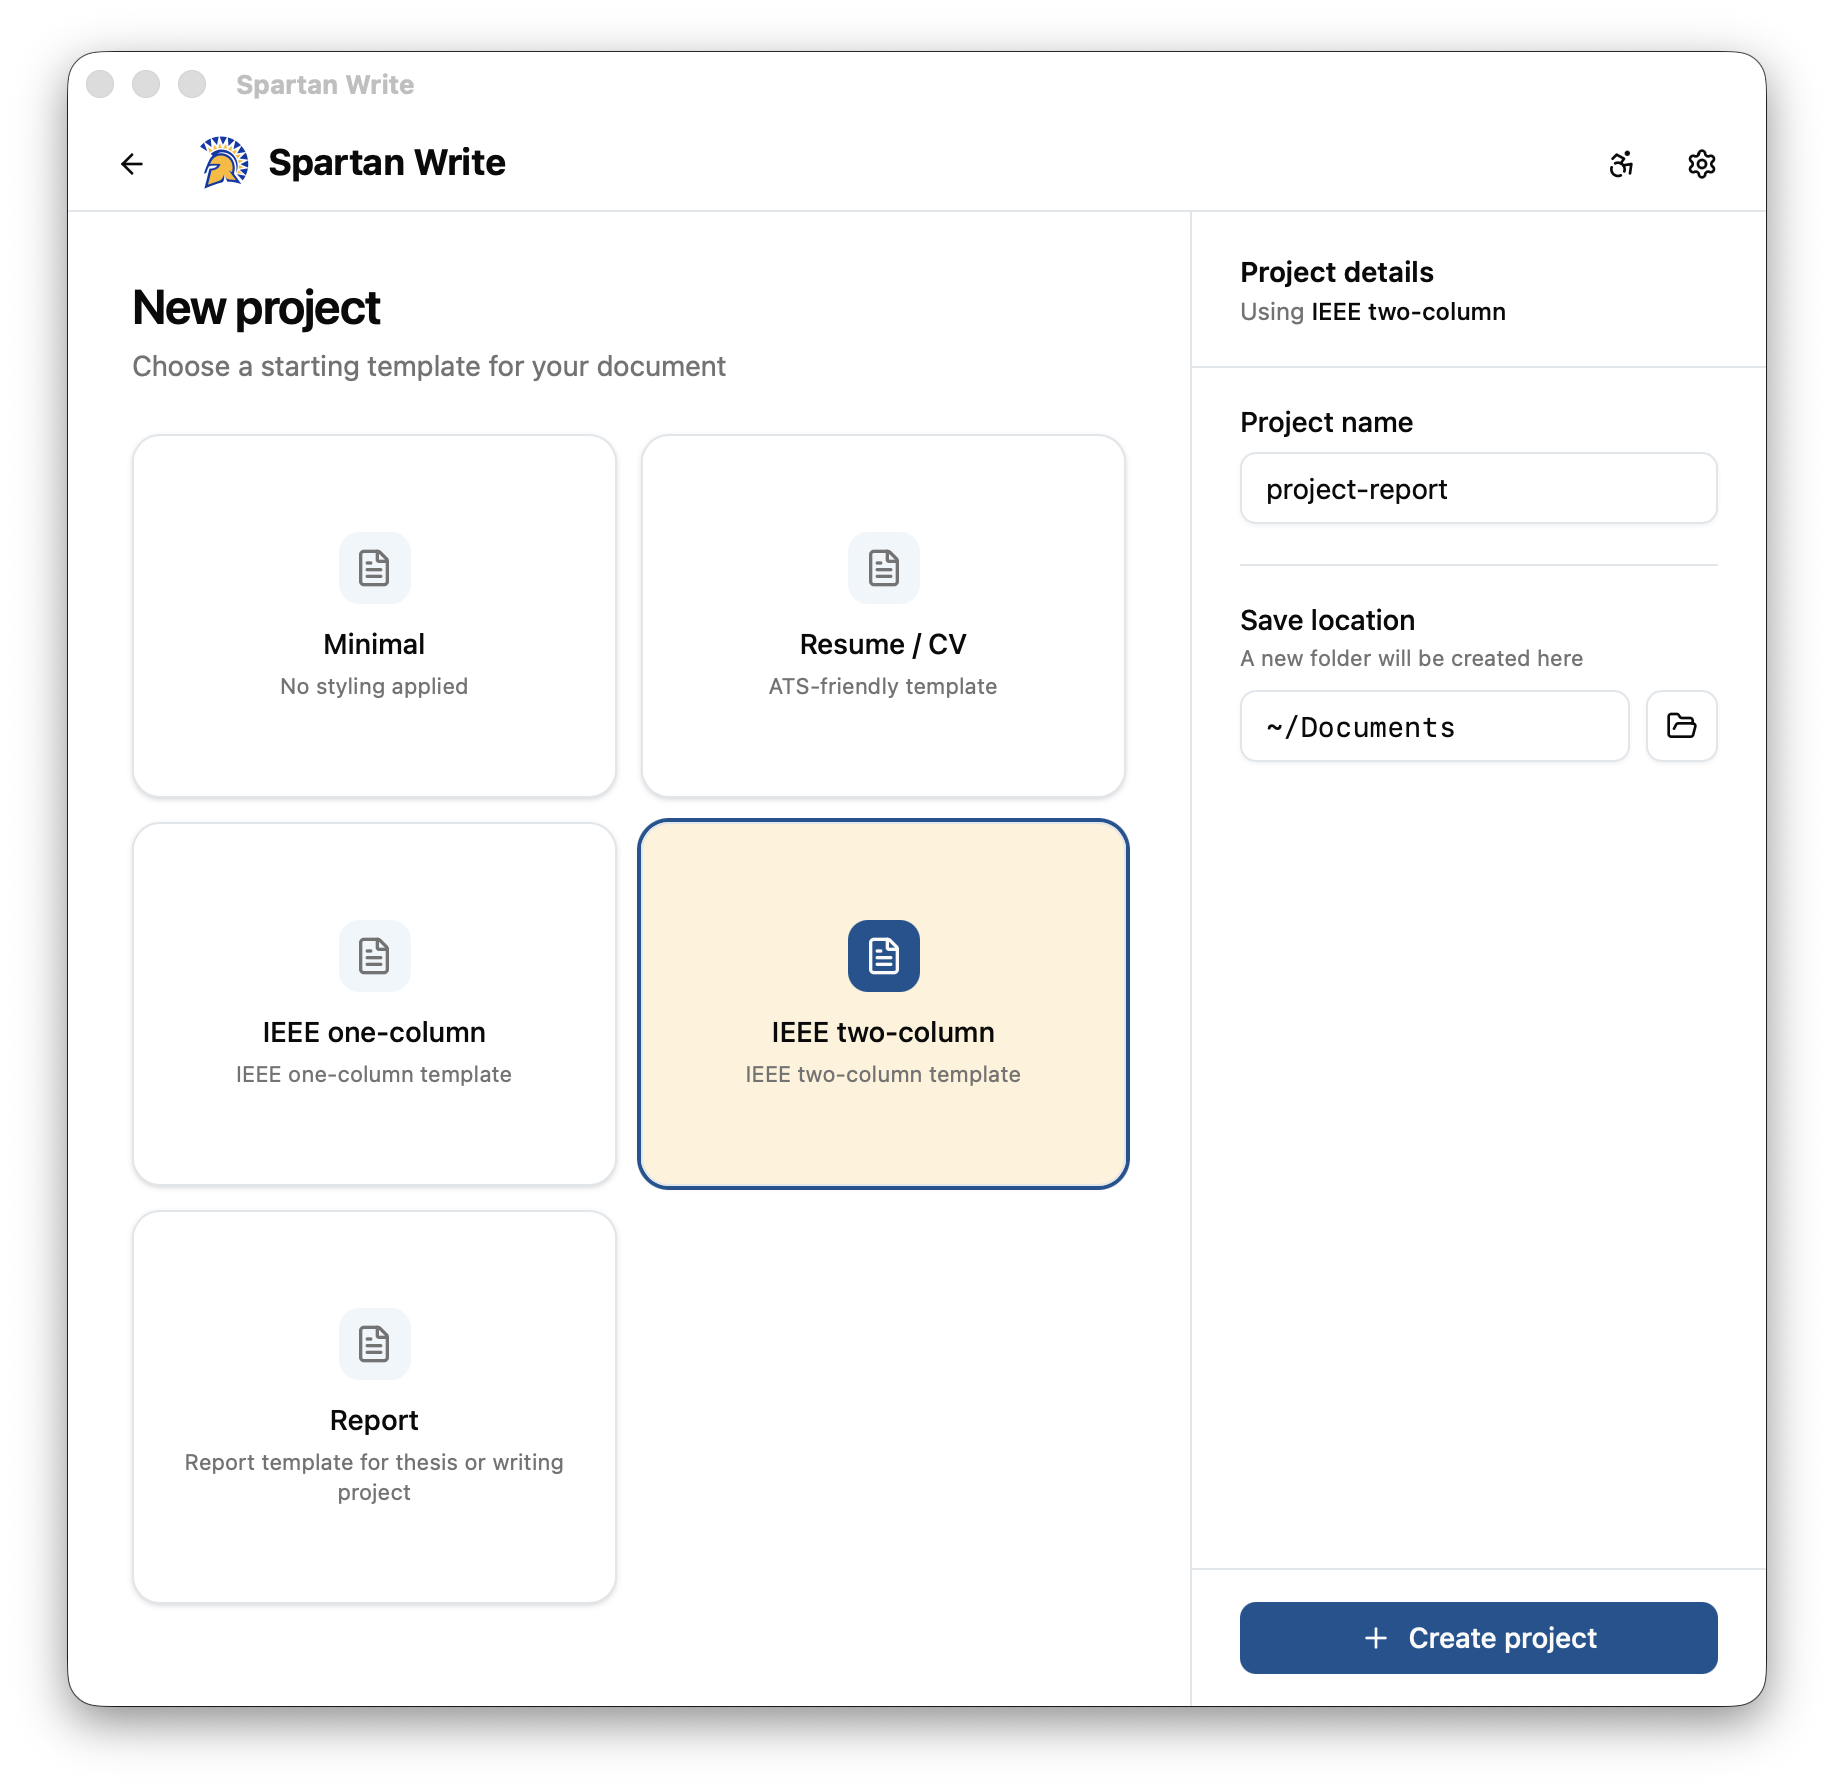
\includegraphics[width=0.67\linewidth]{figures/ui-newproject.png}
    \caption{New project template selection interface}
    \label{fig:ui-newproject}
\end{figure}

\subsubsection{Recent projects page}
Dashboard displaying a list of the user's recently accessed projects with options to open, rename, or delete them, as seen in Figure \ref{fig:ui-dashboard}.

\begin{figure}[htb]
    \centering
    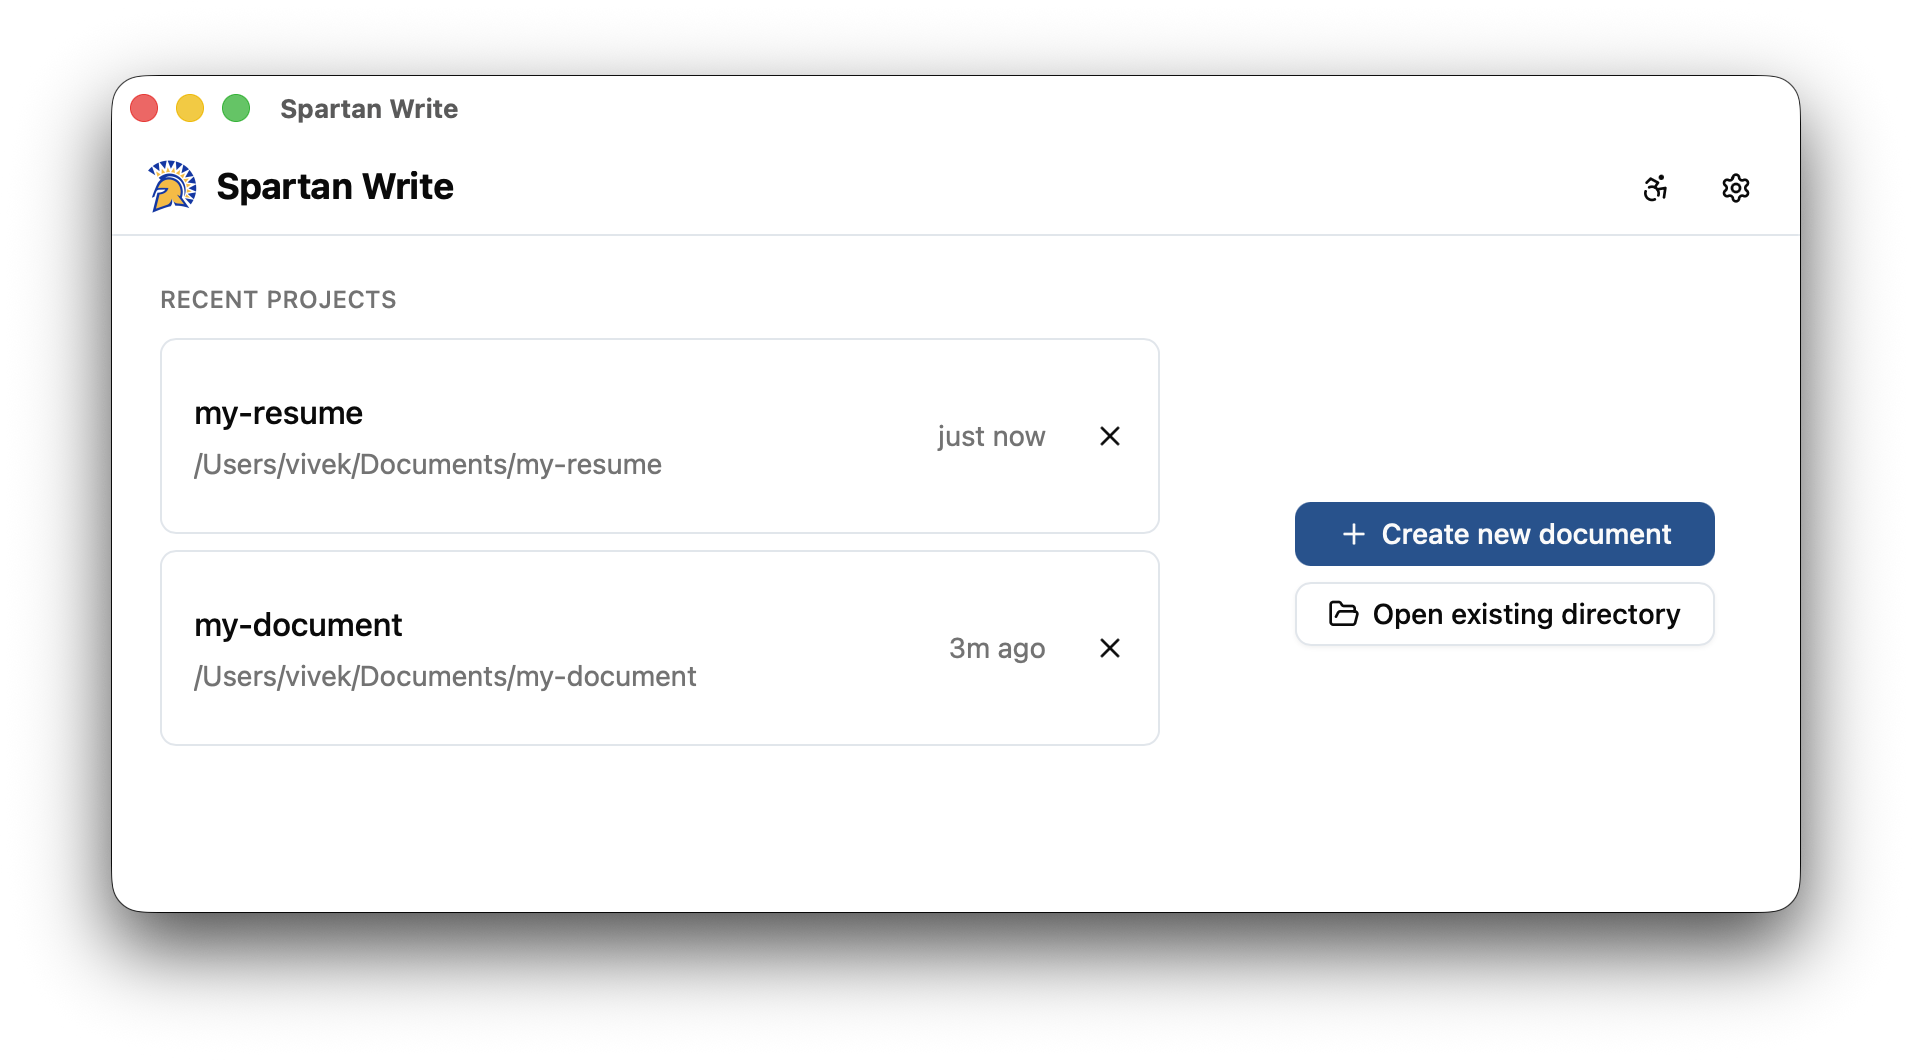
\includegraphics[width=0.67\linewidth]{figures/ui-dashboard.png}
    \caption{Dashboard interface showing recent projects}
    \label{fig:ui-dashboard}
\end{figure}

\subsubsection{Project preview}
The project workspace with the preview interface. The user can see their document draft and interact with a chatbot using the conversation panel, as seen in Figure \ref{fig:ui-docpreview}.

\begin{figure}[htb]
    \centering
    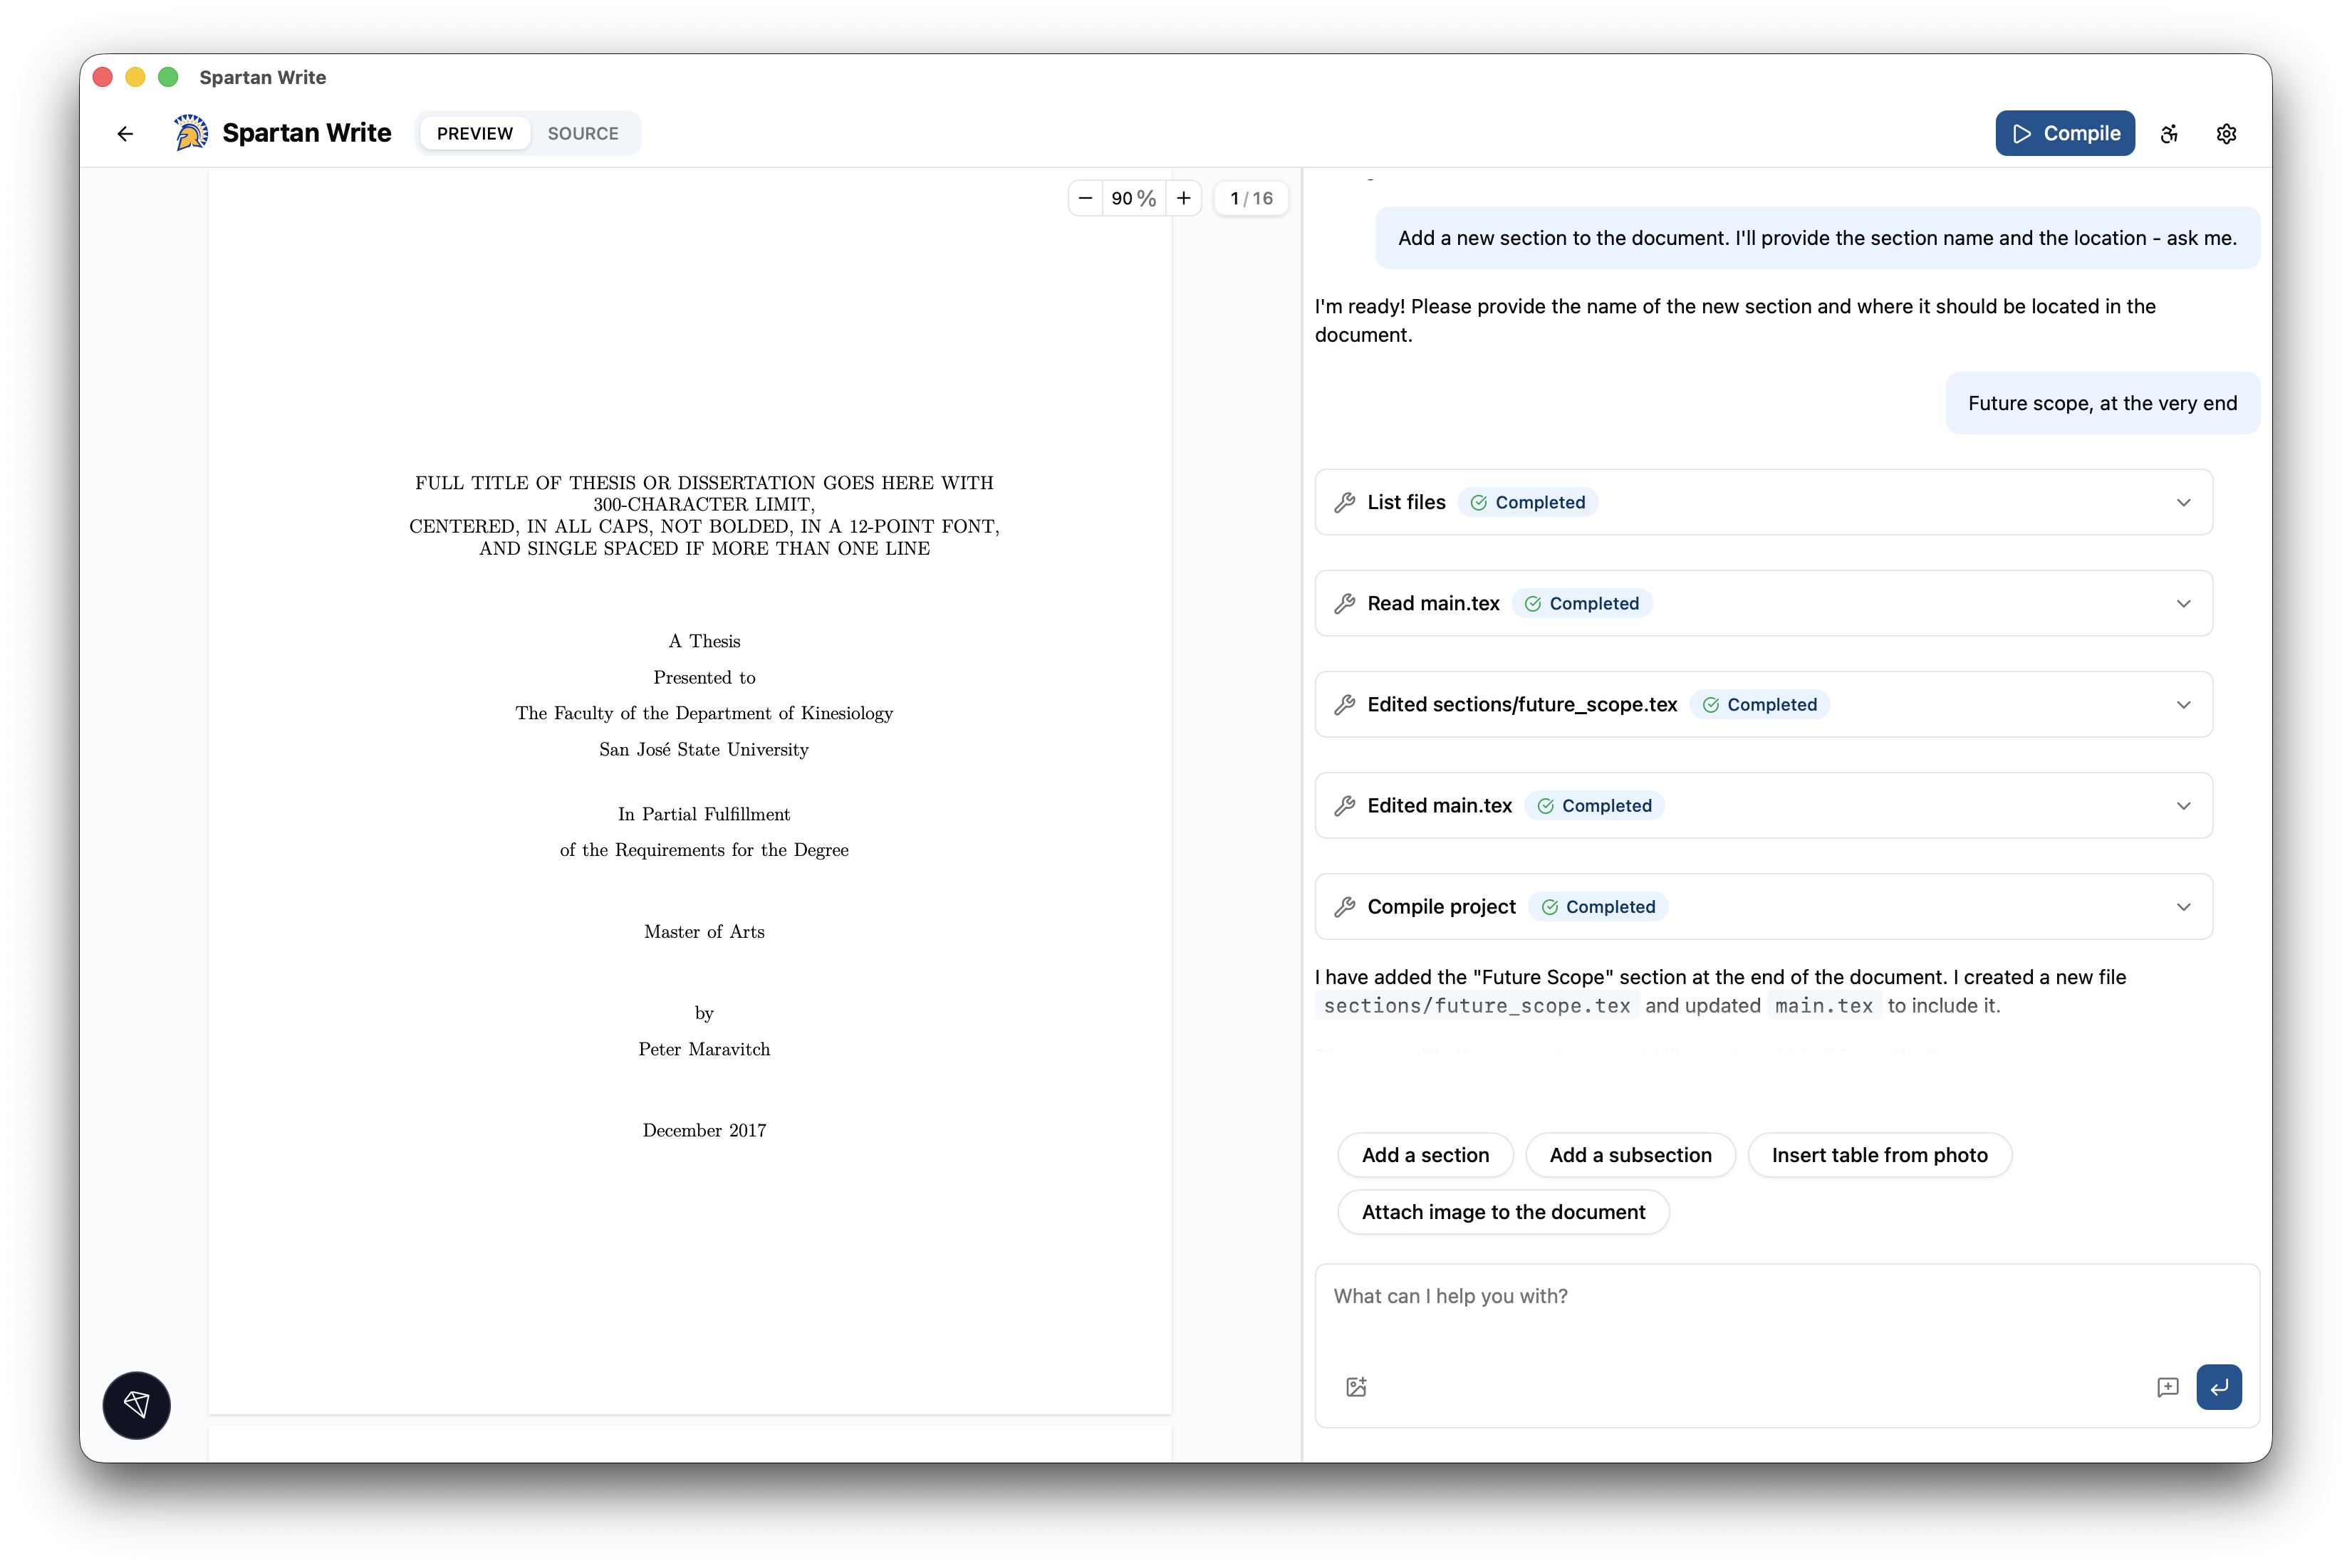
\includegraphics[width=\linewidth]{figures/ui-docpreview.png}
    \caption{Project preview with chat interface}
    \label{fig:ui-docpreview}
\end{figure}

\subsubsection{Source editor}
Text editor for directly editing \LaTeX\ source code with syntax highlighting, line numbers, and code assistance features, as seen in Figure \ref{fig:ui-doceditor}.

\begin{figure}[htb]
    \centering
    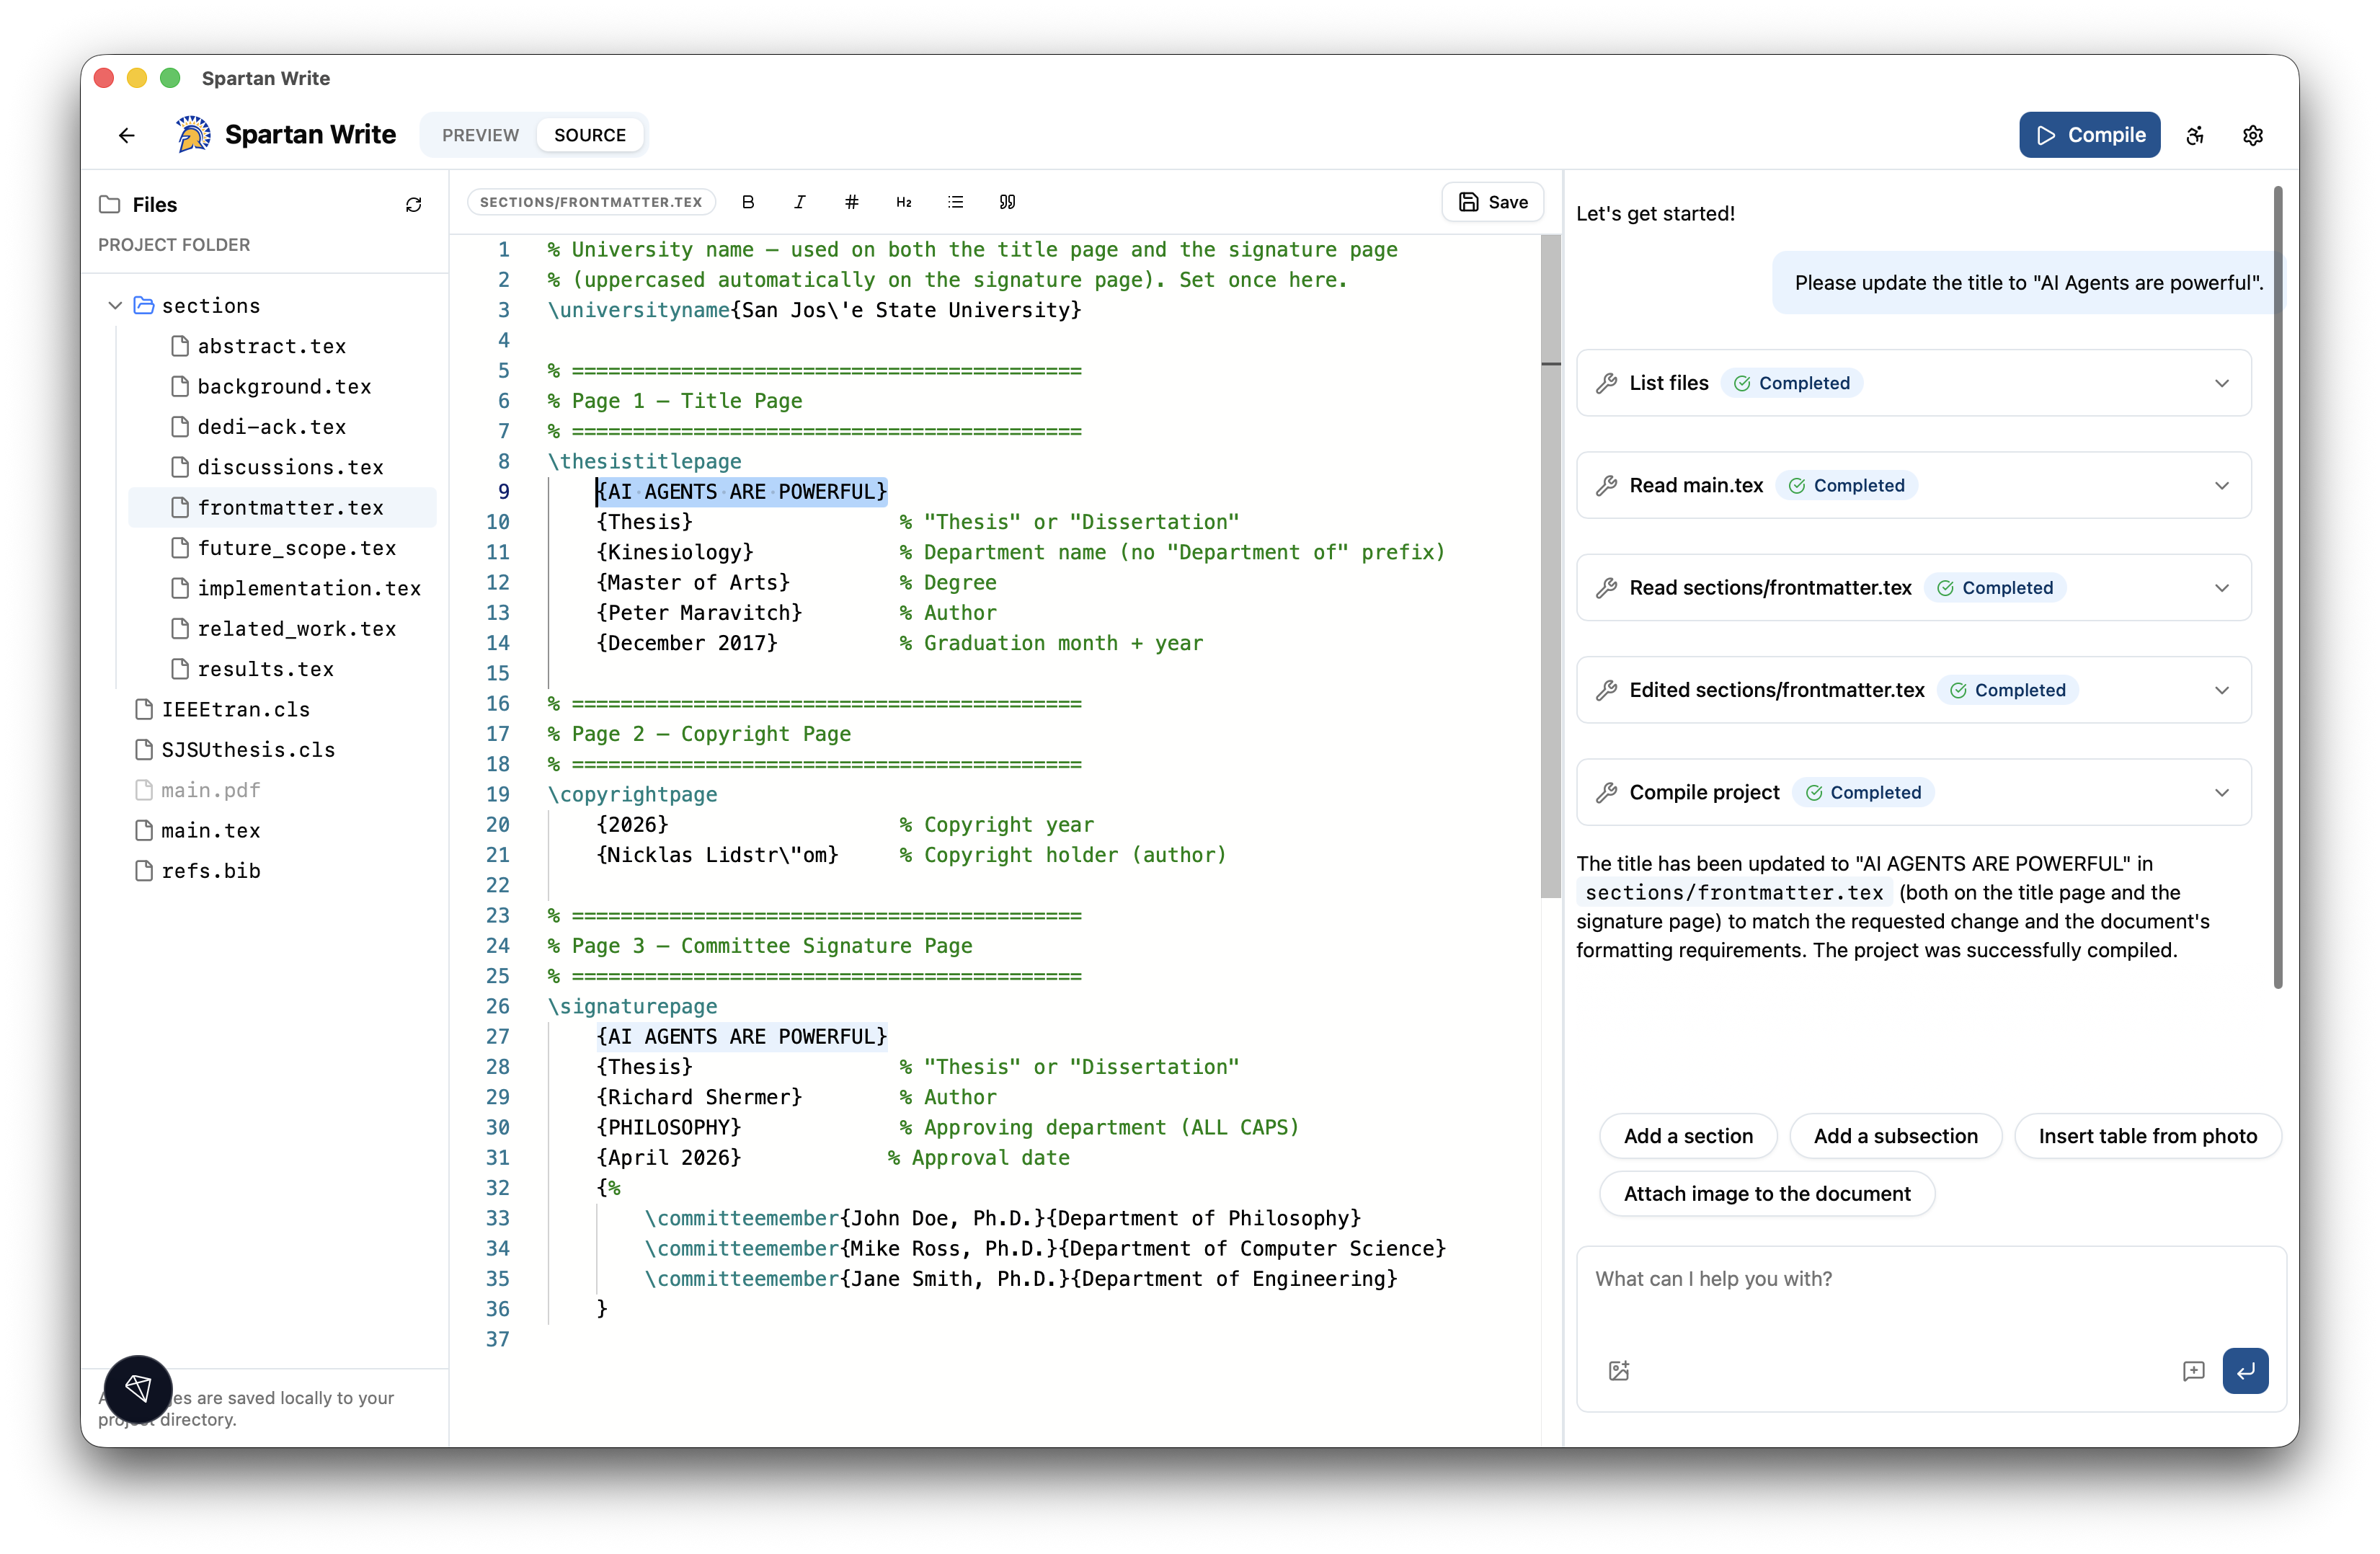
\includegraphics[width=\linewidth]{figures/ui-editor.png}
    \caption{Project source code editor interface}
    \label{fig:ui-editor}
\end{figure}

\subsection{Agent design}

\subsubsection{System prompt}

The agent operates under a comprehensive system prompt that defines its role as a \LaTeX\ assistant capable of understanding user requests and making intelligent document modifications.
The prompt establishes clear guidelines for workflow (list files $\rightarrow$ read $\rightarrow$ edit $\rightarrow$ compile), file organization conventions, and safety principles (minimal changes, user-provided content only, no unsolicited additions).
This prompt-based design ensures consistent, predictable behavior aligned with document integrity best practices.
The complete system prompt can be found in Appendix \ref{apx:system-prompt}

\subsubsection{Architecture}

The agent is implemented as a LangGraph state machine with a deterministic execution graph \cite{langgraph}.
It maintains state across multi-turn conversations, enabling the agent to reference prior context, track intermediate results, and make cumulative edits across multiple user interactions.
The graph structure ensures reliable state transitions and supports checkpoint-based persistence for conversation recovery.

\subsubsection{Tool suite}

The agent has access to seven core tools, as tabulated in Table \ref{tab:agent_tools}.

\begin{table}[htbp]
\centering
\begin{tabular}{|l|p{8cm}|}
\hline
\textbf{Tool name} & \textbf{Description} \\
\hline
\texttt{read\_file\_tool} & Read the contents of any file in the project directory \\
\hline
\texttt{edit\_file\_tool} & Create new files or modify existing files with complete content \\
\hline
\texttt{delete\_file\_tool} & Remove files from the project directory \\
\hline
\texttt{rename\_file\_tool} & Rename or move files within the project, updating all references \\
\hline
\texttt{list\_files\_tool} & Browse and list the project structure recursively or non-recursively \\
\hline
\texttt{compile\_latex\_tool} & Invoke LaTeX compilation and return status and error messages \\
\hline
\texttt{load\_attached\_image\_tool} & Manage image workflows by moving attached images into the figures directory \\
\hline
\end{tabular}
\caption{Tools available to the agent}
\label{tab:agent_tools}
\end{table}

\subsubsection{Tool invocation flow}

When the agent decides to take an action, it invokes the appropriate tool and receives structured output (success/failure, file paths, error messages).
Tool results are fed back into the agent loop, allowing it to respond to outcomes, handle errors, or request clarification from the user.
This interactive loop enables iterative refinement and recovery from failures.

\subsubsection{Compilation}

The agent can invoke \texttt{compile\_latex\_tool} to verify that edits produce valid \LaTeX\ output.
If compilation fails, error messages are captured and the agent can attempt fixes (e.g., correcting syntax errors, fixing citation references).
However, the system enforces a limit on retry attempts (typically 3) within a single user request to prevent infinite loops and resource exhaustion.

\subsubsection{Token usage metrics}

Every agent interaction is tracked and transmitted to PostHog \cite{posthog} to capture comprehensive performance data.
This includes precise token consumption, measuring both input and output volume, tagged with structured metadata such as user ID, model specifications, tool invocations, and session outcomes.
By aggregating these metrics by user, model, and time period, the system provides granular insights into computational costs and infrastructure scaling.
These data points power real-time dashboards that monitor LLM quality and user feedback, directly informing decisions regarding billing logic, usage quotas, and feature development.

\subsubsection{Safety \& ethical constraints}

The agent is designed with built-in safety mechanisms.

\begin{itemize}
    \item All file operations validate paths at the tooling level to prevent escaping the project directory.
    \item The prompt instructs the agent not to add unsolicited content.
    \item Compilation errors trigger error feedback rather than silent failures.
\end{itemize}
These constraints ensure the agent acts as a trusted scribe rather than an autonomous modifier.

\subsection{\LaTeX\ compilation}

The \LaTeX\ compilation subsystem is implemented as a sidecar component \cite{tauri_sidecar}.
The system leverages the Tectonic typesetting engine as its core compilation backend \cite{tectonic}.

Client requests containing the target project directory invoke the Tectonic compiler via subprocess execution with configurable parameters.
Process execution captures both standard output and error streams for diagnostic purposes.
The output PDF file path is displayed to the user upon successful generation.

Compilation can be initiated by either the user or the agent.
In the agent's case, the compilation status and error message are used to iteratively debug and fix the document.

\subsection{User guide}

% TODO

\subsection{Benchmark}

The benchmark module is designed for testing the performance of various language models through the Spartan Write agent.
This is achieved using a reproducible test suite, consisting of a series of test documents and user requests along with different scoring metrics.
The benchmark module consists of four core components:
\begin{itemize}
    \item a CLI runner for orchestration;
    \item a scoring engine for metric evaluation;
    \item SQLite database storage for persistence;
    \item and a Streamlit dashboard for result visualization.
\end{itemize}

\subsubsection{Flow}

The benchmark execution follows a well-defined pipeline.
\begin{itemize}
    \item First, the dataset is loaded into the result directory and the database is initialized.
    \item For each test case, the tool prepares a workspace directory and sends the prompt to the agent server.
    \item After the chat completes, the scoring engine processes results to extract tool usage, duration, and token consumption metrics.
    \item These metrics are stored in the database.
    \item The dashboard then aggregates results from the database and renders interactive visualizations.
\end{itemize}

\subsubsection{Tests design}

% TODO

\subsubsection{Scoring metrics}

The scoring engine evaluates three primary metrics across each benchmark run.
\textbf{Tool use} aggregates tool calls by name and counts invocations per tool type, providing insight into which capabilities the LLM utilized.
\textbf{Chat duration} calculates the time taken for the agent to complete the task. This is primarily used to identify degradation in performance due to LLM updates or provider outages.
\textbf{Token usage} sums input tokens, output tokens, and reasoning tokens across all AI messages, tracking resource consumption.

\section{Dashboard}

The dashboard provides a Streamlit-based interactive web interface \cite{streamlit} that loads all results from the benchmark database and organizes them by model and test job .
Users can filter results by selected models, execution status (pending/complete/failed), error presence, and keyword search across job IDs and test summaries.
The interface renders Plotly charts \cite{plotly} comparing scores across models and showing score distributions for deeper analysis.
Dashboard views also display run-level details including error messages, chat results, and individual run metrics.
Results are grouped by test job ID, with derived fields showing the latest status and scores from the most recent run of each job.
